
\documentclass[10pt,aspectratio=169,mathserif]{beamer}
\usepackage{nju}                 % 1. 主题宏包
\usepackage[UTF8]{ctex}          % 2. 中文支持
\usepackage{amsmath,amsfonts,amssymb,bm} % 3. 数学工具
\usepackage{color}
\usepackage{graphicx}
\usepackage{caption}
\usepackage{subcaption}
\usepackage{booktabs}
\usepackage{diagbox}

% --- 加载biblatex 及其资源文件 ---
\usepackage{natbib}
% --- hyperref放在最后加载---
\usepackage{hyperref,url}

\beamertemplateballitem
% ... 自定义字号,防止原模板中定义与默认字号关键字的冲突,并手动设置悬挂缩进 ...
\DeclareCaptionFont{mytheme}{\scriptsize}
\captionsetup[subfigure]{font=mytheme, format=hang}
\captionsetup[figure]{font=mytheme, format=hang}
\renewcommand{\figurename}{Figure} %图片标题改为英文
\renewcommand{\tablename}{Table} %表头改为英文
\renewcommand{\refname}{References} %参考文献改为英文

%--------------------------------------------------------------
\title{A Leptonic Interpretation of the UHE Gamma-ray Emission from V4641 Sgr}
\author[Su-Yu Wan]{Su-Yu Wan, Jie-Shuang Wang and Ruo-Yu Liu\\
    \textbf{arXiv:2507.02763}\\
    \vspace{1em}
    Speaker: Su-Yu Wan (万苏豫)
  }
\date{2025/08/27}                                                 %日期信息

\iffalse
Hi everyone, I am wan suyu from Nanjing University. The topic of the talk is ...... 
\fi
%--------------------------------------------------------------

\begin{document}
\begin{frame}                                                %生成标题页
\titlepage
\end{frame}				
%--------------------------------------------------------------
\section{Outline}						 %生成提纲页
\begin{frame}
\frametitle{Outline}
\tableofcontents
\end{frame}				
\iffalse
The outline of the speech is listed here.
\fi
%--------------------------------------------------------------
\section{Introduction to V4641 Sgr}
\begin{frame}{Microquasar system: V4641 Sgr}
\begin{itemize}
    \item {Low-mass binary}, a $6.4\pm0.6 M_{sun} $ black hole and a $ 2.9\pm0.4M_{sun} $ companion star.
    \item d = 6.2 kpc, l = 6.77, b = - 4.79. 
    \item Show frequent bursts ($\sim$ 1 - 2 years)
    \item {Experienced a supper-Eddington outburst with X-ray intensities reaching 12.2 Crab.}
    \begin{figure}[ht]
    \centering
    % 使用 subfigure 环境并指定 [t] 选项
    \begin{subfigure}[t]{0.50\linewidth}
        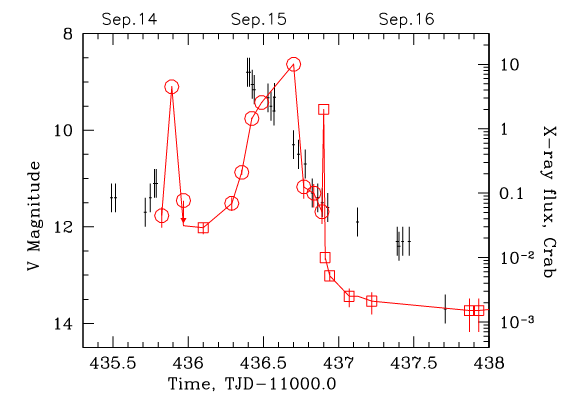
\includegraphics[width=0.7\linewidth]{1999_01.png}
        \caption{The light curves of V4641 Sgr in the optical V-band and in the X-ray band, from \cite{revnivtsev2002v4641sgr}}
        \label{fig:sub1}
    \end{subfigure}%
    \hfill % 在子图之间添加弹性的水平空间
    \begin{subfigure}[t]{0.50\linewidth}
        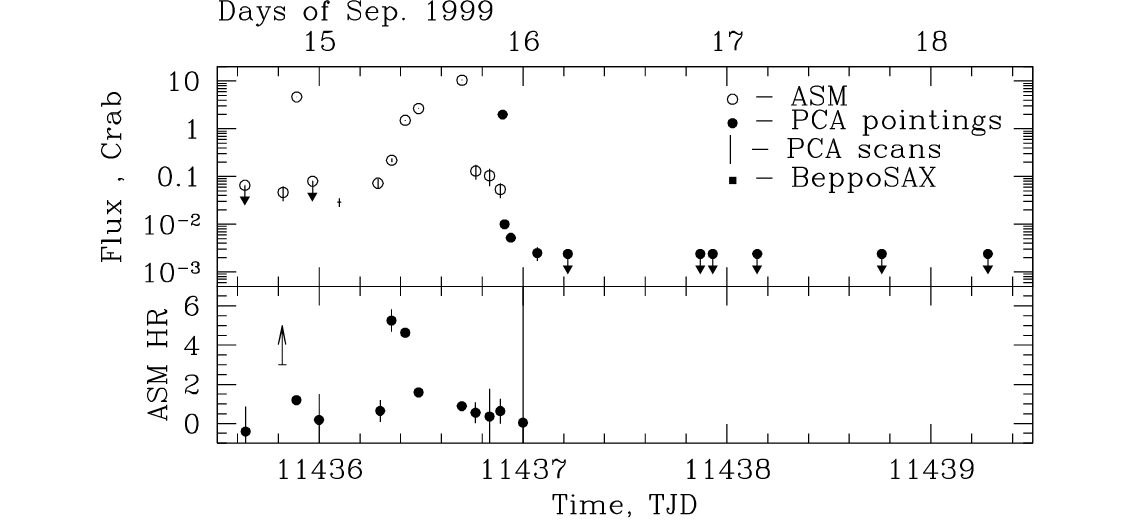
\includegraphics[width=\linewidth]{1999_02.png}
        \caption{The light curve of V4641 Sgr in 1999 according to observations of RXTE and BeppoSAX satellites., from \cite{revnivtsev2002super}}
        \label{fig:sub2}
    \end{subfigure}%
\end{figure}
\end{itemize}
    
\end{frame}


%--------------------------------------------------------------

\begin{frame}
  \frametitle{Picture in TeV - PeV band}

  \begin{itemize}
    \item Evidence for UHE $\gamma$-ray emission from the source (H.E.S.S. + LHAASO + HAWC).
\begin{figure}[ht]
    \centering
    % 使用 subfigure 环境并指定 [t] 选项
    \begin{subfigure}[t]{0.29\linewidth}
        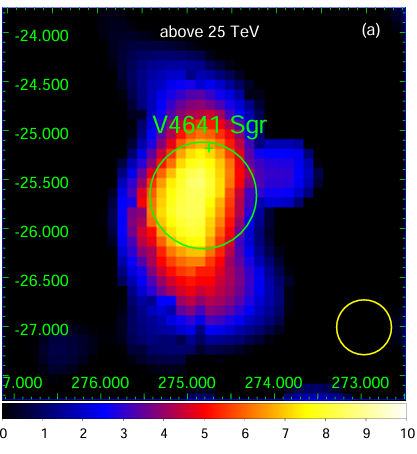
\includegraphics[width=\linewidth]{LHAASO-V4641.png}
        \caption{LHAASO (> 25 TeV),\\from \cite{lhaaso2024ultrahigh}}
        \label{fig:sub1}
    \end{subfigure}%
    \hfill % 在子图之间添加弹性的水平空间
    \begin{subfigure}[t]{0.30\linewidth}
        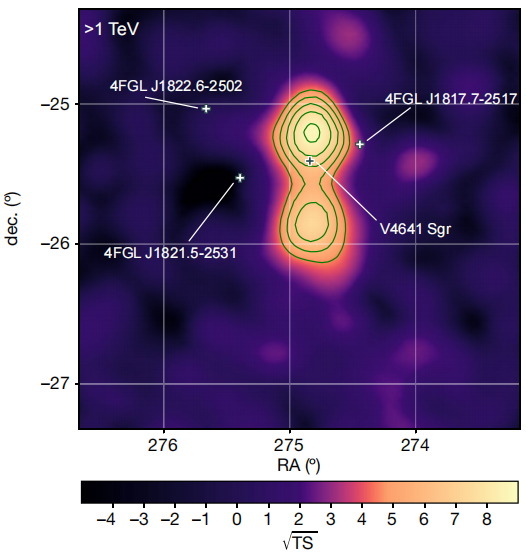
\includegraphics[width=\linewidth]{HAWC4641_1.png}
        \caption{HAWC (> 1 TeV), from \cite{alfaro2024ultra}}
        \label{fig:sub2}
    \end{subfigure}%
    \hfill
    \begin{subfigure}[t]{0.30\linewidth}
        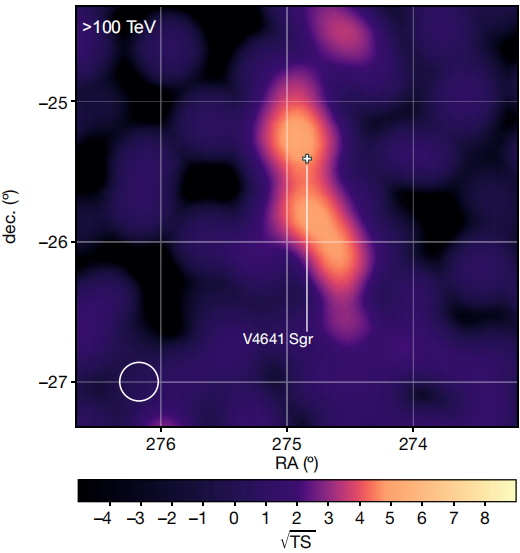
\includegraphics[width=\linewidth]{HAWC4641_2.png}
        \caption{HAWC (> 100 TeV), from \cite{alfaro2024ultra}}
        \label{fig:sub3}
    \end{subfigure}
    \label{fig:subcaption-align}
\end{figure}

\item Elongated morphology ($\sim$ 100 pc) + Ultrahigh energy photons ($\sim$ 0.8 PeV).
\item Two point sources or an extended source ?
  \end{itemize}
\end{frame}

\iffalse
V4641 Sgr is a microquasar system consisting of a low-mass BH and a B-type companion star. It experienced a famous super-Eddington outburst in Nineteen Ninety-nine, with X-ray intensities reaching 12.2 Crab and a radio jet also occurred. Last year, Evidence for ultra-high energy gamma-ray emission from the source is detected with various experiments, including HESS, LHASSO and HAWC. All of them finds that the UHE source takes a elongated morphology and LHAASO detected UHE photons whose energy reaches around 0.8 PeV.
\fi
%--------------------------------------------------------------

\begin{frame}{Possible explanations}
 \begin{columns}[T] % [T] 选项让两栏内容顶部对齐
    % --- 左栏:放置图片 ---
    \begin{column}{0.5\textwidth} 
        \begin{figure}
        \centering
        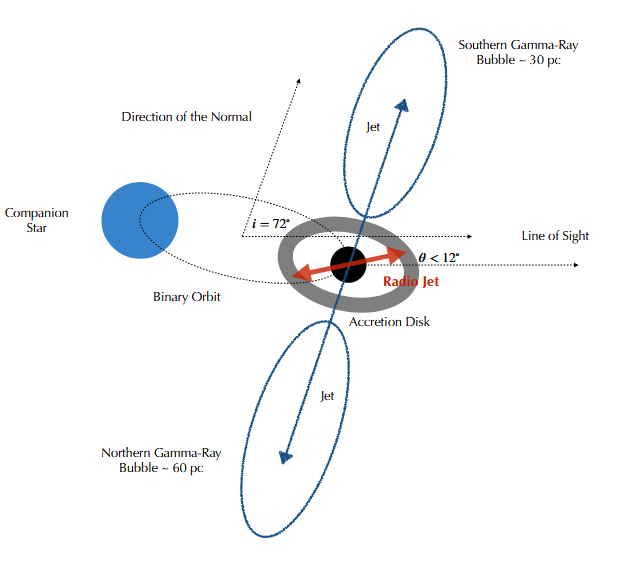
\includegraphics[scale=0.4]{Alfaro.png}
        \caption{Two - lobe scenario. \citep{alfaro2024ultra}}
        \label{fig:confine}
        \end{figure}
        \begin{itemize}
            \item No sufficient medium.
            \item Acceleration may not be efficient enough.
        \end{itemize}
    \end{column}
    % --- 右栏:放置列表 ---
    \begin{column}{0.5\textwidth} % 指定右栏宽度为页面宽度的 50%
        \begin{figure}
        \centering
        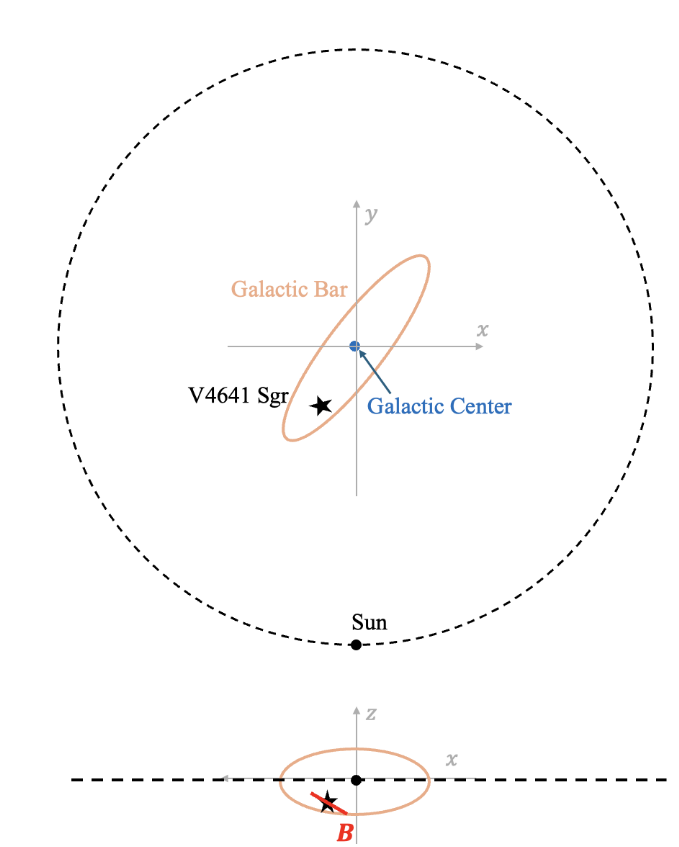
\includegraphics[scale=0.25]{Nerenov.png}
        \caption{Escaping cosmic ray particles. \citep{neronov2025multimessenger}}
        \label{fig:confine}
        \end{figure}
      \begin{itemize}
          \item Total proton energy $\sim$ $10^{50}\, \rm erg$
          \item Long-term injection of protons is required.
      \end{itemize}
    
    \end{column}    
  \end{columns}
    
\end{frame}



%--------------------------------------------------------------
\section{Leptonic modelling}
\begin{frame}
  \frametitle{Leptonic modelling}
	\begin{block}{Klein-Nishina effect would steepen the spectrum + More efficient cooling}
	    \begin{itemize}
	        \item A hard spectrum is needed.
             \item A `distributed' acceleration mechanism is required (in jet/outflow).
	    \end{itemize}
	  \end{block}
    Stochastic acceleration (STA) + Shear acceleration (SHA), described by Fokker - Planck equation:
	$\frac{\partial n(\gamma,t)}{\partial t}=\frac{1}{2}\frac{\partial}{\partial \gamma}[\langle \frac{\Delta \gamma^2}{\Delta t} \rangle \frac{\partial n(\gamma,t)}{\partial \gamma}]-\frac{\partial}{\partial \gamma}[(\langle \frac{\Delta \gamma}{\Delta t} \rangle-\frac{1}{2}\frac{\partial}{\partial \gamma}\langle \frac{\Delta \gamma^2}{\Delta t} \rangle+\left \langle \dot{\gamma_c} \right \rangle)n(\gamma,t)]-\frac{n(\gamma,t)}{t_{\rm esc}}+Q(\gamma,t)$.
 \begin{columns}
     \begin{column}{0.5\textwidth}
            \begin{itemize}
             \item Steady-state solution ($\partial n$/$\partial t$ = 0):\\
             \begin{equation*}
                N(\gamma)=
                \left \{
                \begin{array}{l@{\quad}l}
                \begin{aligned}
                &K_0\gamma^{1-q}&  \gamma<\gamma_{\rm eq}\,, \\
                &K_2\gamma^{s_-}{_1F}_1\left(a_-,b_-;z\left(\gamma\right)\right)& \gamma_{\rm eq}\le \gamma<\gamma_{\rm rsn}\,,\\
                &D_2\gamma^{p_{\rm -}} &\gamma_{\rm rsn}\leq\gamma\,.
                %\end{cases}K_1\gamma^{s_+}{_1F}_1\left(a_+,b_+;z\right)\\&+, D_1\gamma^{p_{\rm +}} + 
                \label{e29}
                \end{aligned}
                \end{array}
                \right.
              \end{equation*}
           \end{itemize}
     \end{column}

     \begin{column}{0.5\textwidth}
        \begin{figure}
        \centering
        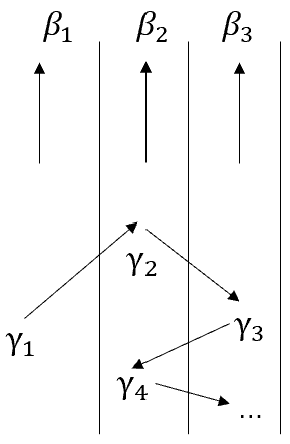
\includegraphics[scale=0.4]{shearacc.png}
        \caption{Sketch of shear acceleration.}
        \label{fig:confine}
        \end{figure}
     \end{column}
 \end{columns}
\end{frame}

\iffalse
Here we use a leptonic model to explain the observed emission. Assuming that the observed structure is a jet composed of a spine with constant speed and a velocity-shear layer, whose length is around 100 pc. Electrons in the jet will experience both stochastic and shear acceleration caused by the interactions between the particles and MHD waves along with the background flow, and they can be accelerated to a high energy, making it possible to reproduce UHE photons via inverse compton processes regardless of KN effect. By solving the Fokker-Planck equation, which describes the particle distribution in stochastic processes, we can get the electron spectrum. Here the velocity distribution is assumed to be a linear one, and the radius of the jet's spine equals to $\eta R_{\rm jet}$. Here are some basic parameters for the model. It is necessary to mention that when $r_{\rm L}$>$\Lambda_{\rm max}$, the loss of low-order wave-particle interactions would make the electrons move ballistically, causing a larger MFP.
\fi
%--------------------------------------------------------------
  \begin{frame}
  \frametitle{Parameter constraints}
  \begin{columns}
  \begin{column}{0.5\textwidth}
	 \begin{enumerate}
	    \item The maximum luminosity: \\
             $L_{\rm kin}$ $\leq$ $L_{\rm Edd}$
             
	    \item Hillas criterion ($r_{\rm L}$ < $R_{\rm jet}$):\\
        The maximum energy is defined by $\gamma_{\rm Hillas} = \frac{eB_0R_{\rm jet}}{m_{\rm e} c^2}\,.$
	    \item Electrons' mean free path (MFP) ($\lambda$ < $R_{\rm jet}$):\\
        The maximum energy is defined by $\gamma_{\rm MFP} = \frac{eB_0}{m_{\rm e} c^2}\left( \xi \Lambda_{\rm max}^{1-q}R_{\rm jet}\right)^{\frac{1}{2-q}}\,.$
	\item Cooling rates should not be too high: $t_{\rm acc, SHA} \leq t_{\rm cool}\,.$  
      \end{enumerate}
  \end{column}
  \begin{column}{0.5\textwidth}
      \begin{figure}
        \centering
        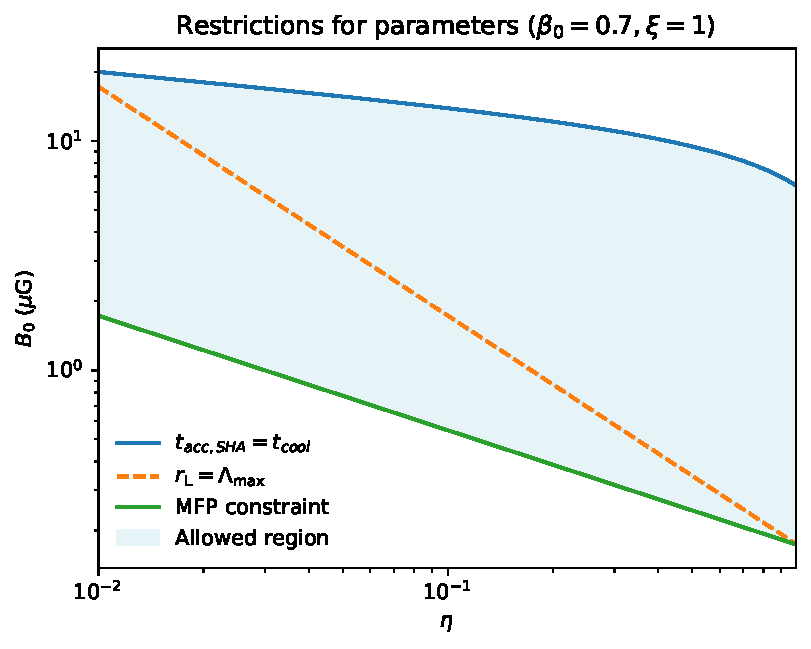
\includegraphics[scale=0.35]{xi=1_beta=0.7.pdf}
        \caption{$\eta-B_0$ planes which show the potential parameter sets under two confinements: $c\tau_{\rm sc} \le R_{\rm jet}$ and $t_{\rm acc,\rm SHA} \le t_{\rm cool}$, with $\beta_0$ = 0.7, q=5/3, $R_{\rm jet}$ = 5 pc and $\gamma$ = 0.8 ${\rm PeV}/\left({m_{\rm e} c^2}\right)$. The orange dashed line indicates the limit for the 1st-order resonance and the shaded area represents the allowed parameter regions when $\xi=1$. 
        \label{fig:confine}}
        \end{figure}
    \end{column}
    \end{columns}
    \end{frame}
\iffalse
After considering all terms above, the equation can be solved analytically. The electron spectrum is a piece-wise function containing three power-law components. The low-energy spectrum is composed of electrons accelerated via STA, whose index is 1-q, and the high-energy spectrums are composed of electrons accelerated via SHA. The spectrum should be continuous and additional constraints are applied to primarily constrain the parameters: Firstly, the maximum luminosity is smaller than the Eddington luminosity; Secondly, the Hillas criterion should be satisfied. Thirdly, the MFPs of electrons are smaller than the radius of the jet and at last, the cooling rates should not be too high.
\fi

%--------------------------------------------------------------
\section{Results}
\begin{frame}
  \frametitle{Results: Data fitting}
    \begin{columns}[T] % [T] 选项让两栏内容顶部对齐
    % --- 左栏:放置图片 ---
    \begin{column}{0.5\textwidth} 
      \begin{figure}
        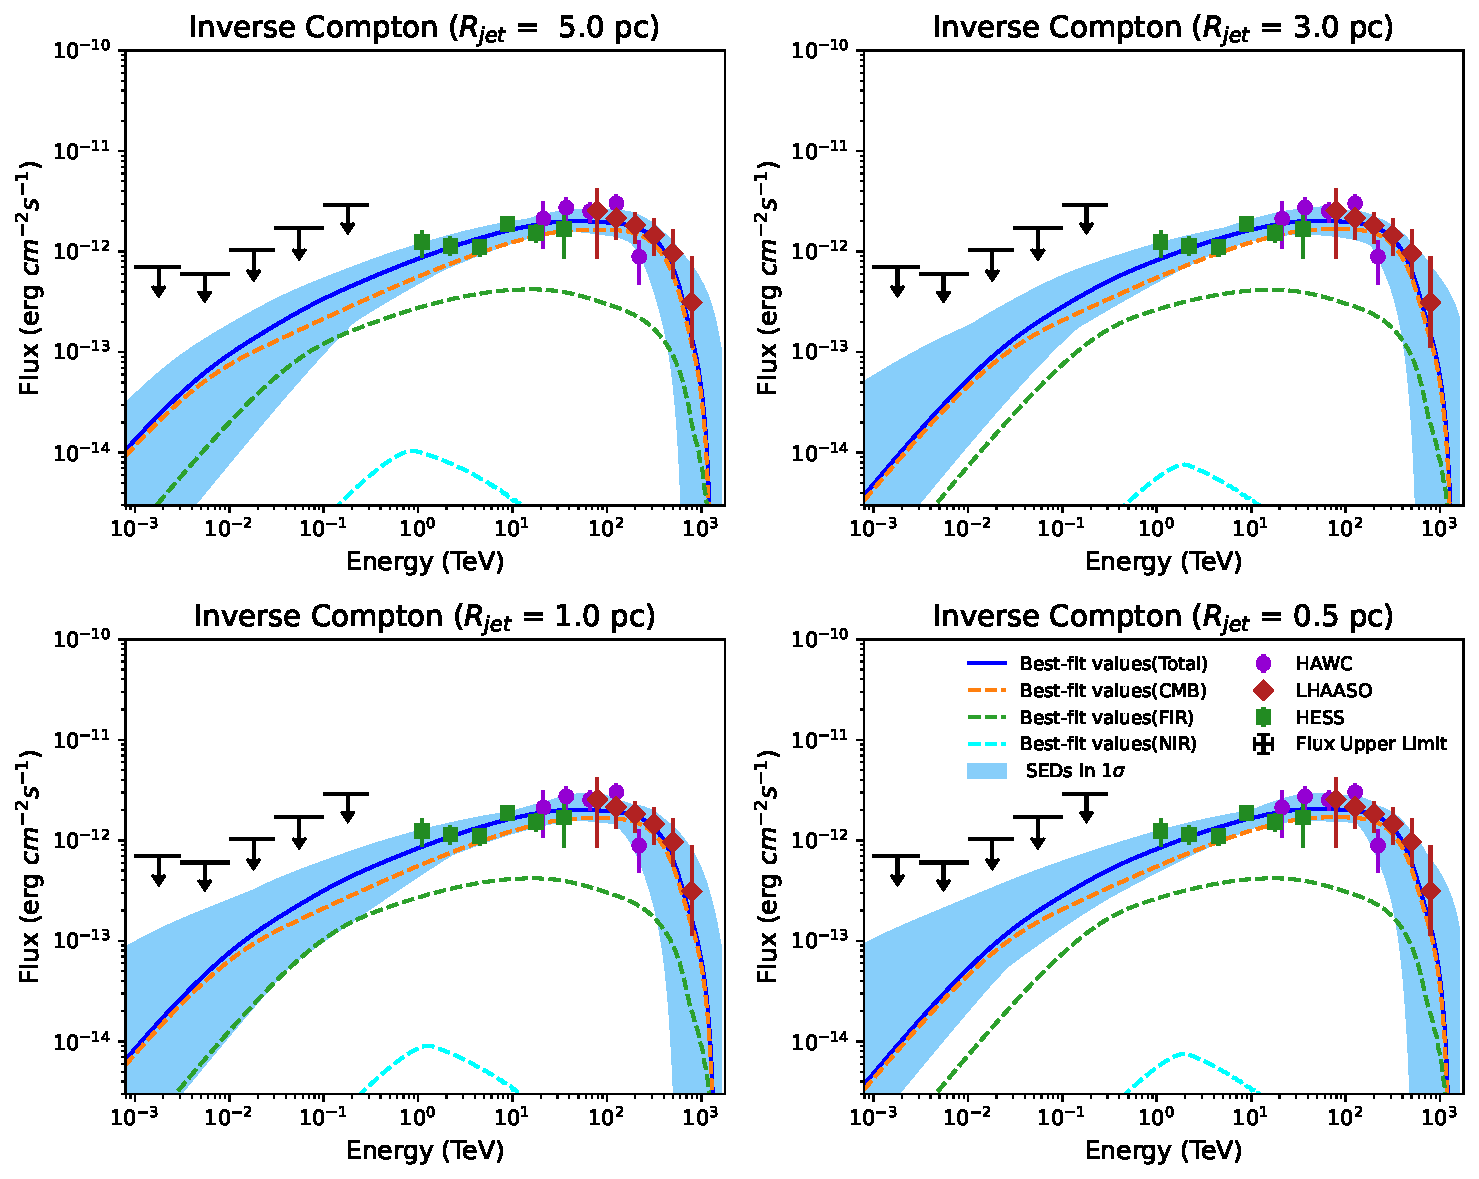
\includegraphics[width=\textwidth]{IC_all_HESS_q=1.6666666666666667.pdf}
        \caption{The fitting results for the UHE spectrum of V4641 Sgr (derived from MCMC).}
        \label{fig:confine}
      \end{figure}
    \end{column}
    % --- 右栏:放置列表 ---
    \begin{column}{0.5\textwidth} % 指定右栏宽度为页面宽度的 50%
      \begin{itemize}
          \item Three photon fields, considering the optical depth $\tau_{\gamma \gamma}\,.$
          \item MCMC is used to fit the data with various $R_{\rm jet}$ values.
      \end{itemize}

    \begin{table}
        \caption{Best-fit parameters from $\chi^2$ tests}
        \setlength{\belowcaptionskip}{0pt}
        \label{tab:paras1}
        \resizebox{1.0\textwidth}{!}{
        \begin{tabular}{lcccc}
        \toprule
         & \multicolumn{4}{c}{Jet radius $R_{\rm jet}$} \\
        \cmidrule(lr){2-5}
        Parameters & 5 pc & 3 pc & 1 pc & 0.5 pc \\ 
        \midrule
        $\log B_0$ ($\mu$G) 
        & $-0.32^{+0.20}_{-0.35}$ & $-0.02^{+0.13}_{-0.40}$ & $0.49^{+0.07}_{-0.45}$ & $0.73^{+0.10}_{-0.40}$  \\
        
        $\eta$ ($R_{\rm shear}/R_{\rm jet}$)  
        & $0.38^{+0.39}_{-0.13}$ & $0.29^{+0.43}_{-0.07}$ & $0.28^{+0.46}_{-0.05}$ & $0.30^{+0.44}_{-0.06}$ \\
        
        $\beta_0$ (Spine velocity)  
        & $0.70^{+0.21}_{-0.08}$ & $0.64^{+0.25}_{-0.05}$ & $0.62^{+0.28}_{-0.02}$ & $0.65^{+0.25}_{-0.03}$ \\
        
        $\log N_{\rm tot}$ (Norm.) 
        & $46.90^{+0.72}_{-1.02}$ & $46.42^{+1.47}_{-0.43}$ & $46.59^{+1.95}_{-0.49}$ & $46.42^{+2.17}_{-0.25}$   \\
        
        $\chi^2/$d.o.f. & 13.5/12 & 13.5/12 & 13.4/12 & 13.5/12  \\
        \bottomrule
        \end{tabular}
        }
        \end{table}

    \begin{itemize}
        \item $B_0$ depends on the radius of the jet.
    \end{itemize}
    
    \end{column}    
  \end{columns}
\end{frame}
\iffalse
Next we calculate the IC emission produced by the electrons and three background photon fields, including CMB, FIR and NIR. MCMC is used to fit the observed data under various $R_{\rm jet}$ values. The results are shown in the figure and the table. We find that the leptonic emission can explain the observation well, and the magnetic field around the source strongly depends on the radius of the jet. The predicted magnetic field becomes lower when the radius of the jet increases.
\fi
%--------------------------------------------------------------

\begin{frame}
\frametitle{Results: X-ray emission}
\begin{columns}[T] % [T] 选项让两栏内容顶部对齐
    % --- 左栏:放置图片 ---
    \begin{column}{0.5\textwidth} 
      \begin{figure}
        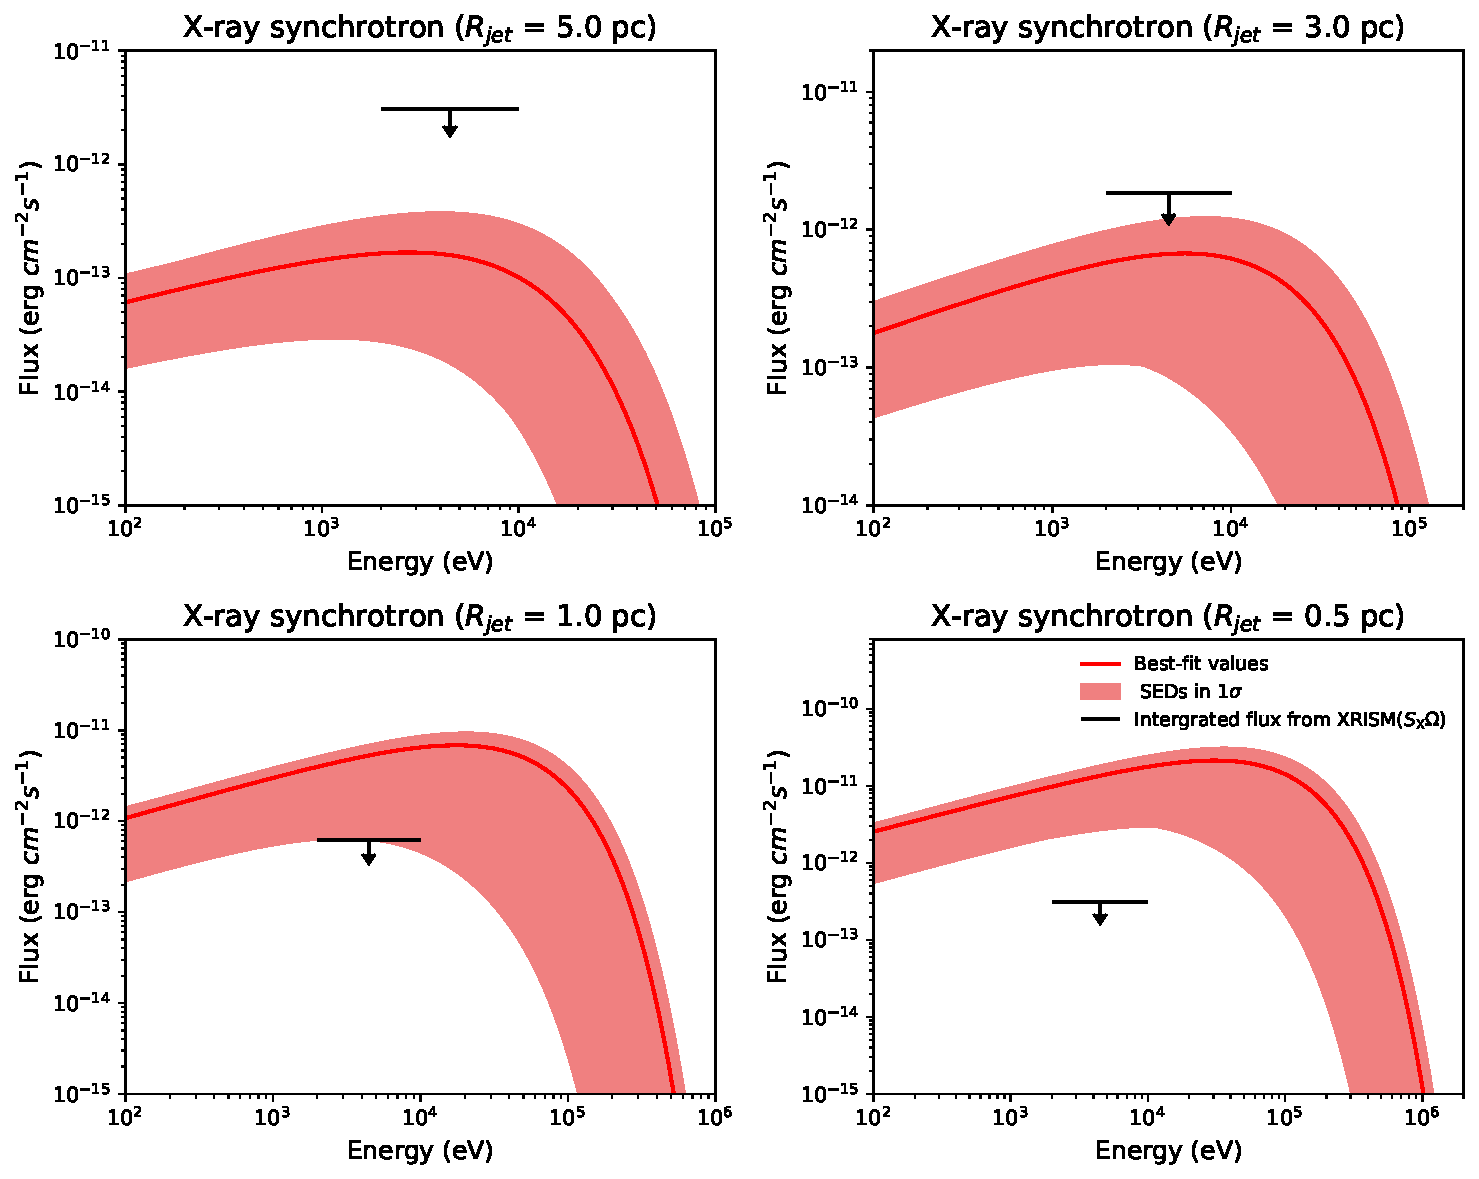
\includegraphics[width=\textwidth]{SYN_all_HESS_flat_q=1.6666666666666667.pdf}
        \caption{The synchrotron emission produced by the same electron population responsible for the UHE gamma-ray emission.}
        \label{fig:confine}
      \end{figure}
    \end{column}

    % --- 右栏:列举条目 ---
    \begin{column}{0.5\textwidth}
    \begin{figure}
        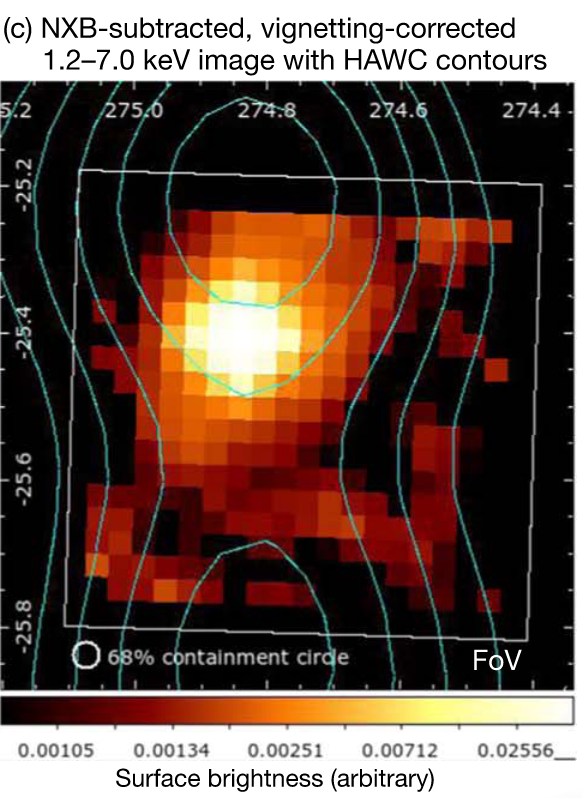
\includegraphics[width=0.35\textwidth]{XRISM.png}
        \caption{Recent observation of XRISM has revealed an extended X-ray source around V4641 Sgr (\citep{suzuki2025detection}}
        \label{fig:confine}
      \end{figure}
    \begin{itemize}
        \item $R_{\rm jet}>1\,$pc is favored for this model, and the constraint may be relaxed if future observations detect X-ray emission from the region outside its field of view.
    \end{itemize}
    \end{column}
\end{columns}
\end{frame}

\iffalse
We also calculate the X-ray synchrotron emission produced by the same electron population responsible for the UHE gamma-ray emission. A recent observation of XRISM has revealed an extended X-ray source around V4641 Sgr, which can help to further constrain the magnetic field. We find that $R_{\rm jet}$ > 1 pc is required for this model to make the magnetic field around a micro-gauss scale. The constraint may be relaxed if ......
\fi


%--------------------------------------------------------------
\section{Disussions}
\begin{frame}
  \frametitle{Discussions - Dependence on the turbulence spectrum}
\begin{columns}[T] % [T] 选项让两栏内容顶部对齐
    % --- 左栏:放置图片 ---
    \begin{column}{0.5\textwidth} 
      \begin{figure}
        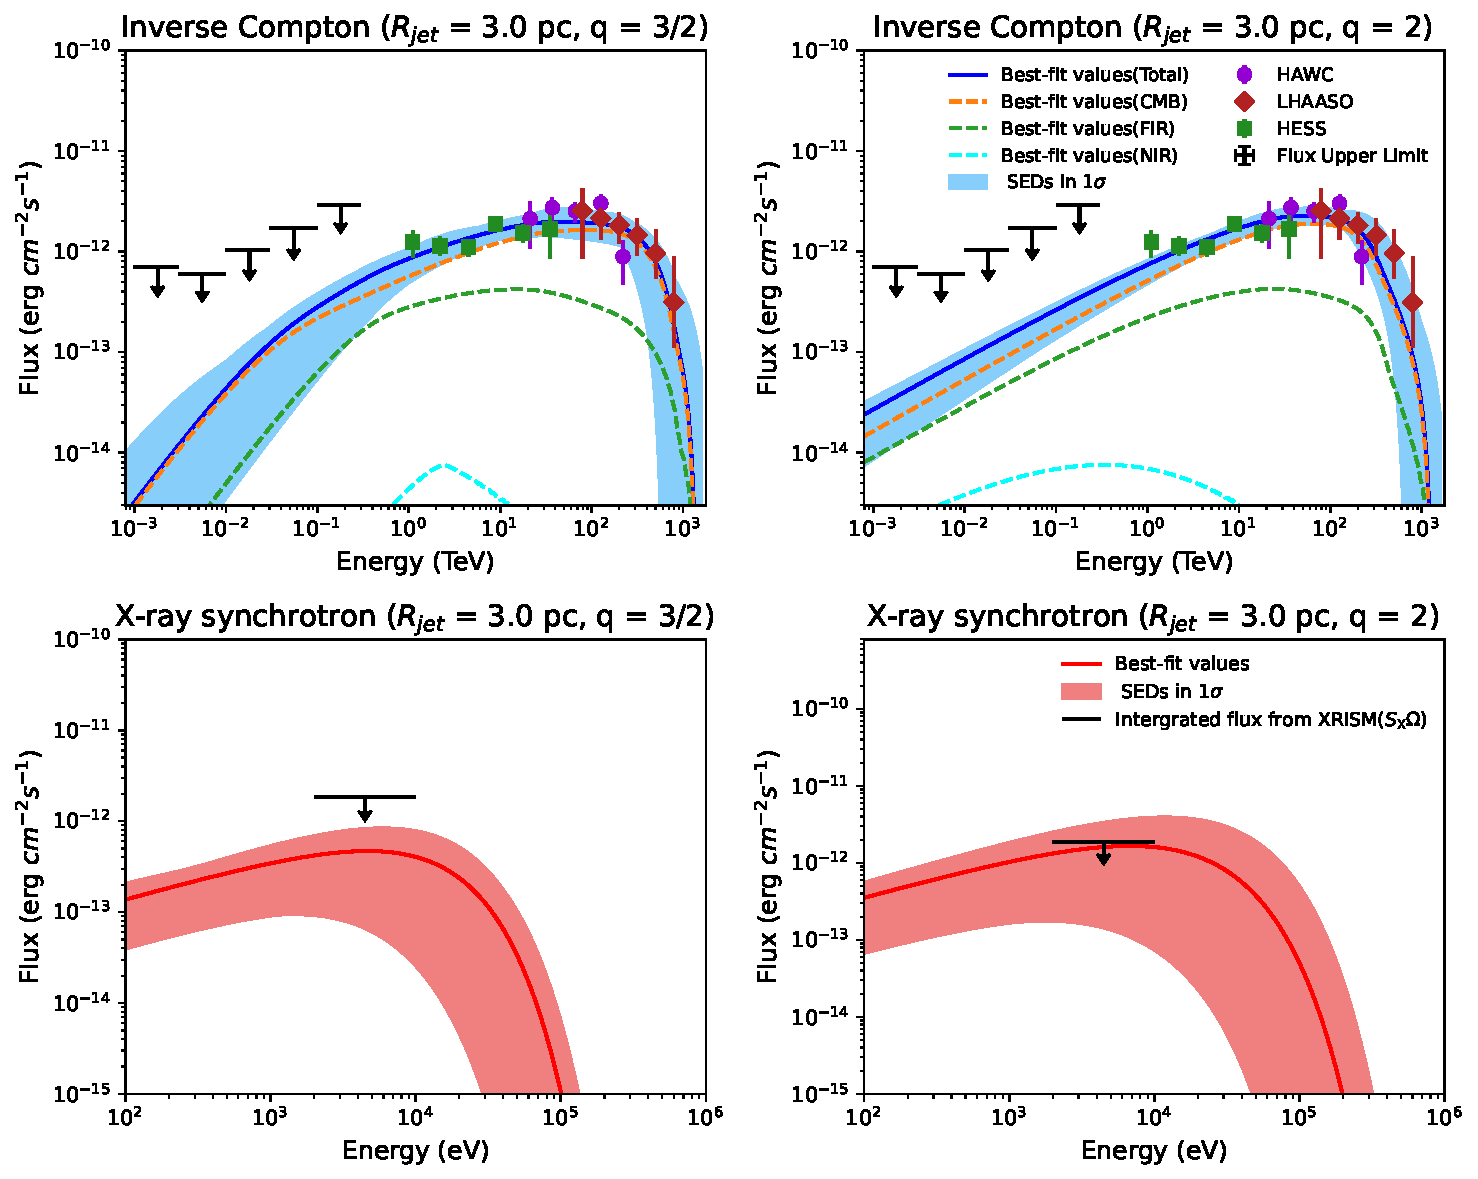
\includegraphics[width=\textwidth]{SYNIC_all_HESS_flat_q=1.pdf}
        \caption{The fitting results for the UHE spectrum and predicted X-ray synchrotron flux, with different types of turbulence.}
        \label{fig:confine}
      \end{figure}
    \end{column}

    % --- 右栏:列举条目 ---
    \begin{column}{0.5\textwidth} 
    \begin{itemize}
        \item The main parameters do not vary much from those with $q=5/3$,  except for $N_{\rm tot}$ when $q=2$.
        \item The electron kinetic luminosity of the jet ($\epsilon_{\rm e} $) keeps $\sim 10^{35 - 36}\,\rm erg\,s^{-1}$
    \end{itemize}

\begin{table}
\caption{Best-fit parameters from $\chi^2$ tests\label{tab:paras2}}
\resizebox{0.7\textwidth}{!}{
\begin{tabular}{lcc}
\toprule
 & \multicolumn{2}{c}{Type of turbulence} \\
\cmidrule(lr){2-3}
Parameters & $q = 3/2$ & $q = 2$  \\ 
\midrule
$\log B_0$ ($\mu$G) 
& $-0.09^{+0.10}_{-0.36}$ & $0.16^{+0.14}_{-0.49}$   \\

$\eta$ ($R_{\rm shear}/R_{\rm jet}$)  
& $0.42^{+0.31}_{-0.20}$ & $0.11^{+0.21}_{-0.01}$  \\

$\beta_0$ (Spine velocity)  
& $0.78^{+0.15}_{-0.10}$ & $0.38^{+0.25}_{-0.01}$  \\

$\log N_{\rm tot}$ (Norm.) 
& $46.51^{+0.84}_{-0.76}$ & $51.67^{+0.50}_{-1.41}$    \\

$\chi^2/$d.o.f. & 13.6/12 & 13.4/12   \\
\bottomrule
\end{tabular}
}
\end{table}

\begin{itemize}
    \item A highly relativistic jet is required if q $\rightarrow$ 1.
\end{itemize}

    \end{column}
\end{columns}

\end{frame}

\iffalse
Furthermore, we look into how the turbulence spectrum influences the results. We find that the main parameters do not vary much from those with Kolmogorov jet. However, when q = 2, $N_{\rm tot}$ will significantly increase for there are more low-energy electrons. However, the electron's kinetic luminosity of the jet stays nearly unchanged. When q gets closed to 1, a highly relativistic jet is required.
\fi
%--------------------------------------------------------------

\begin{frame}
  \frametitle{Discussions - Possibilities for STA to work solely}
	\begin{columns}[T] % [T] 选项让两栏内容顶部对齐
    % --- 左栏:放置图片 ---
    \begin{column}{0.5\textwidth} 
      \begin{figure}
        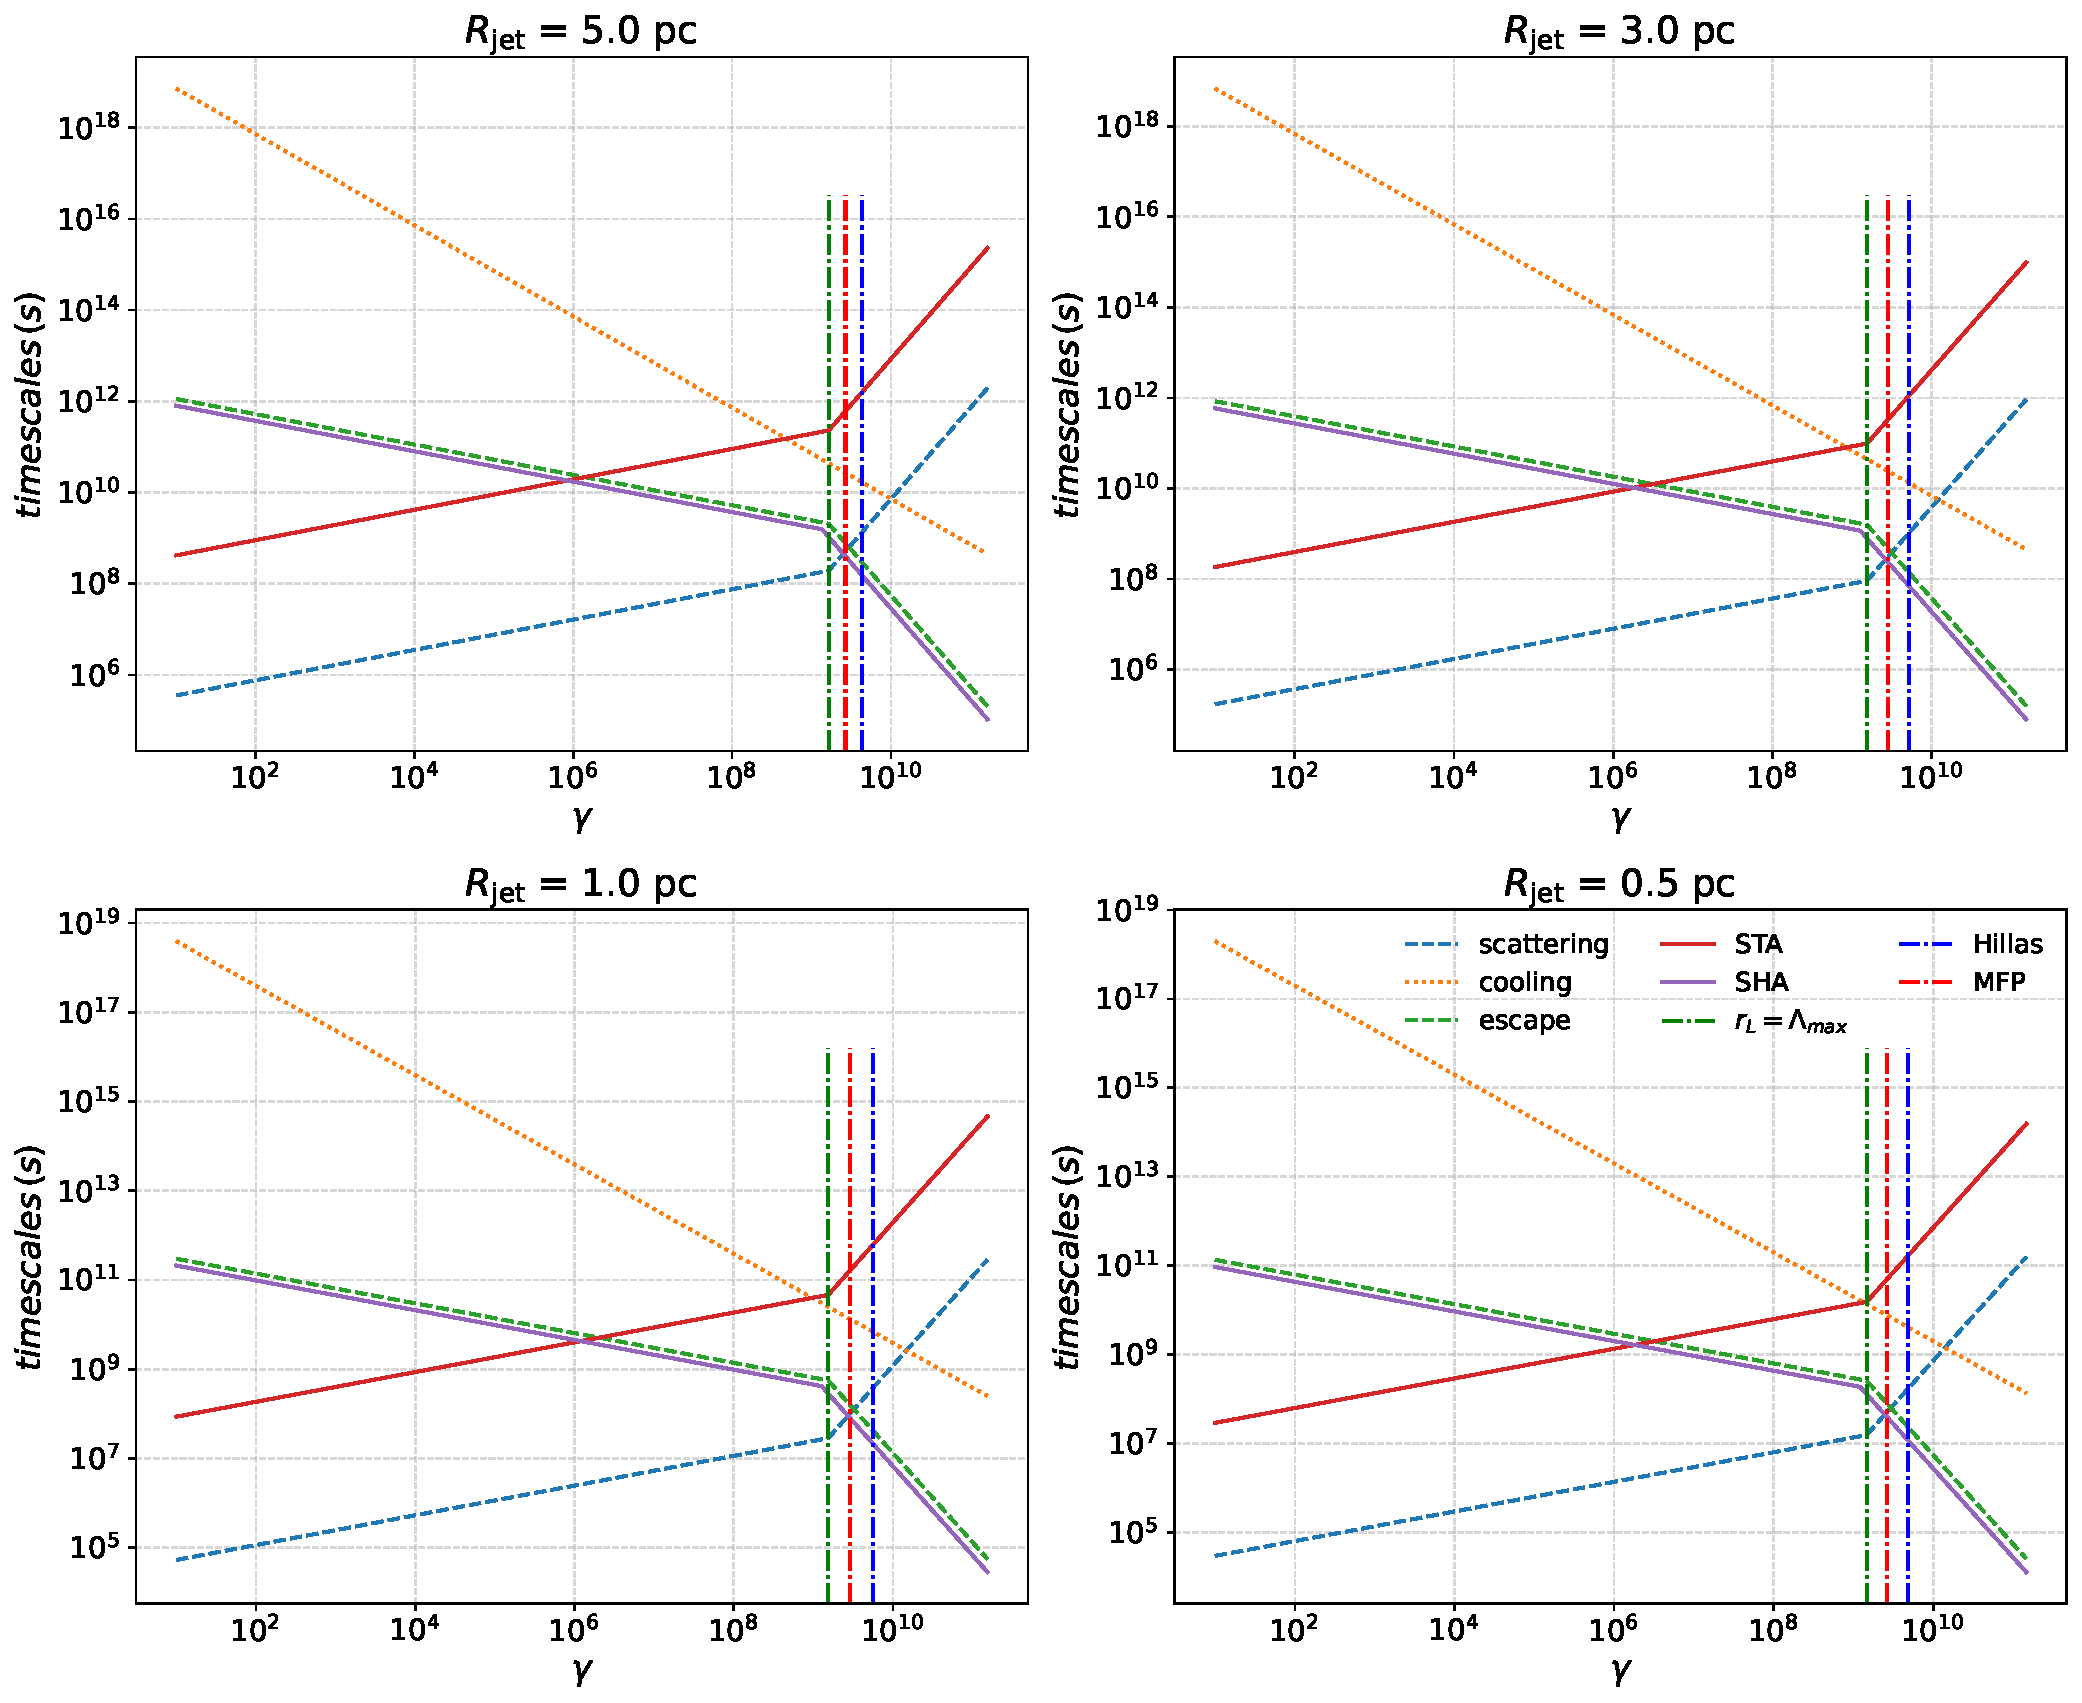
\includegraphics[width=\textwidth]{Tscales_all.pdf}
        \caption{Timescales for different processes with the best-fit parameters from MCMC fittings.}
        \label{fig:confine}
      \end{figure}
    \end{column}
    % --- 右栏:列举条目 ---
    \begin{column}{0.5\textwidth} 
    \begin{itemize}
        \item From MCMC results (q = 5/3), the escape of accelerated electrons is efficient.
        \item Generally, the accelerated particle spectrum of STA is too hard to explain the measured spectrum of V4641~Sgr.
        \item However, the spectrum can be softened when q = 2 (Both $t_{\rm acc,STA}$ and $t_{\rm esc}$ become energy-indepedent).
        \item To accelerate the electrons to $\sim$ 0.8 PeV, a very low baryon density of the jet is needed to overcome cooling:
    \end{itemize}
    \vspace{-9pt}
    \begin{align*}
        \xi = 1,\, B_0=2\,\rm \mu\text{G},\, &\Lambda_{\rm max}=0.8\,{\rm PeV}/\left(eB_0\right) \\
        &\downarrow\\
        \vspace{-8pt}
        \beta_{\rm A}>0.09\, , &n_{\rm p}<2.4\times 10^{-8}\,\rm cm^{-3}
    \end{align*}
        
    \end{column}
\end{columns}
\end{frame}
%--------------------------------------------------------------

\section{Conclusions}
\begin{frame}
  \frametitle{Conclusions}
  \begin{itemize}
      \item A jet with velocity-shear flows have the potential to accelerate electrons to $\sim$ PeV level via shear acceleration mechanism, given favorable parameters.

      \item The magnetic field inside the jet under four chosen values of $R_{\rm jet}$ are constrained at $\mu$G level and the bulk jet speed is around $0.6\rm c-0.7\rm c$.

      \item The X-ray synchrotron emission from the same electron population, whose total flux in $2-10$\,keV could range from $10^{-13}$ to $10^{-12}\rm \,erg\,cm^{-2}\,s^{-1}$. Recent observations of XRISM on V4641~Sgr may favor $R_{\rm jet} > 1$\,pc. 

      \item The model would predict a truly elongated morphology of the UHE gamma-ray source, and future X-ray observations of full coverage of the UHE source may give a stronger constraint on the model.
  \end{itemize}
\end{frame}

%--------------------------------------------------------------
\begin{frame}
\frametitle{Regards}
\Huge{\centerline{Thanks for listening !}}
\centerline{\small Please feel free to contact me: \textbf{\small \url{sywan2002@smail.nju.edu.cn}}
}
\end{frame}


%--------------------------------------------------------------
%\char65f8
\bibliographystyle{plainnat}
\bibliography{myrefs}

\begin{frame}{Backup page 1}
\begin{figure}[ht]
    \centering
        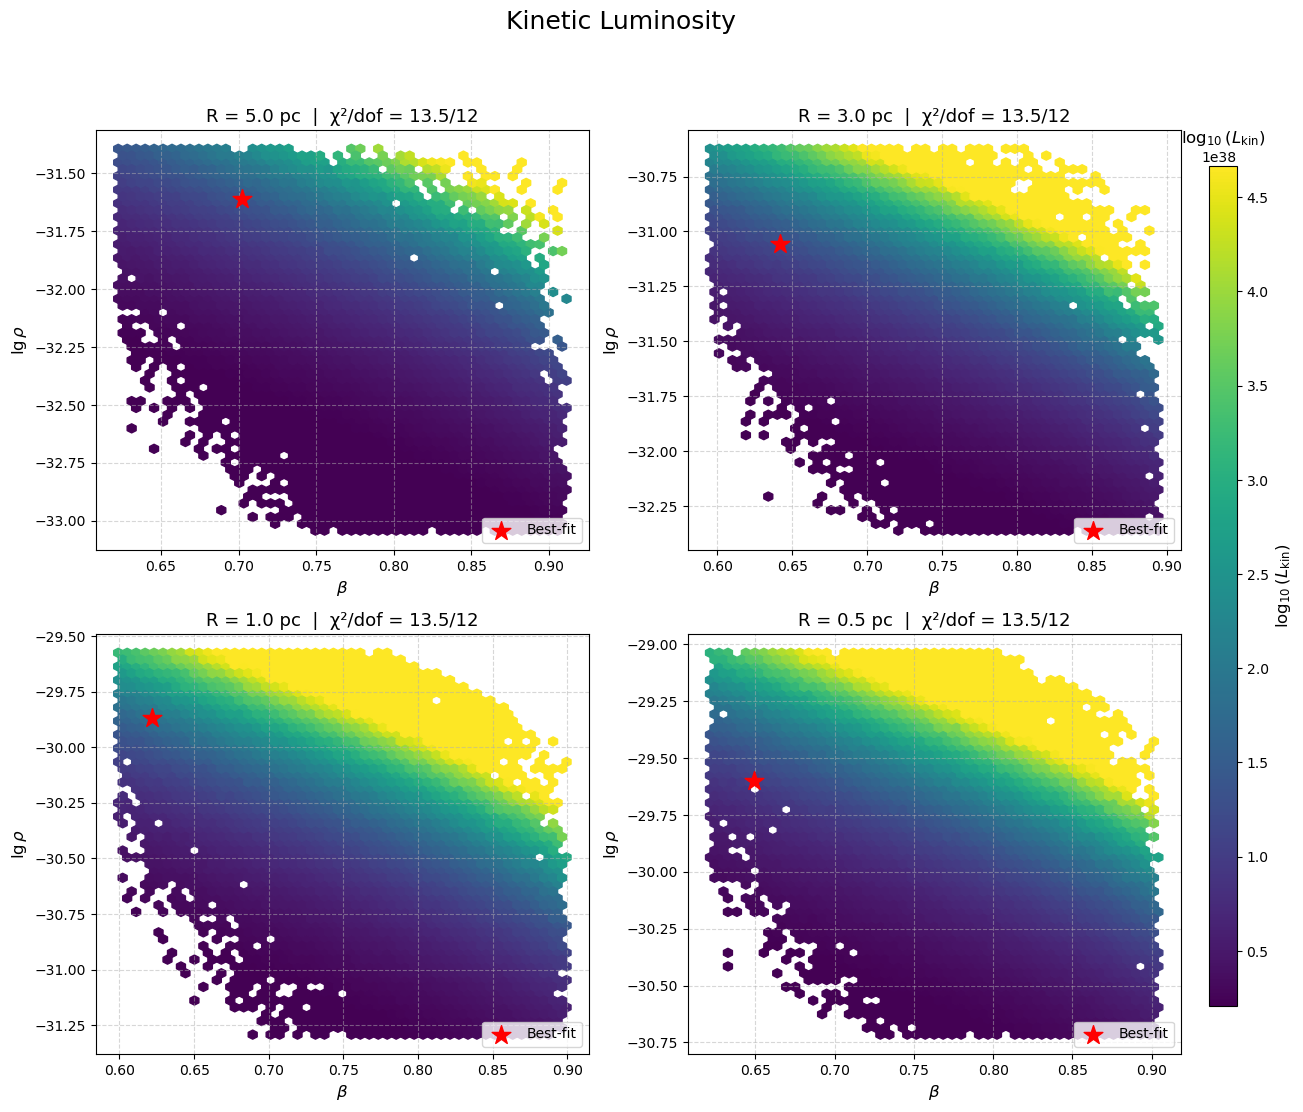
\includegraphics[width=0.5\linewidth]{proton_kin.png}
        \caption{Protons' kinetic luminosity for all samples within 1-$\sigma$ statistical uncertainties.}
        \label{fig:sub1}
\end{figure}
\end{frame}
%--------------------------------------------------------------

\begin{frame}{Backup page 2}
\begin{figure}[ht]
    \centering
        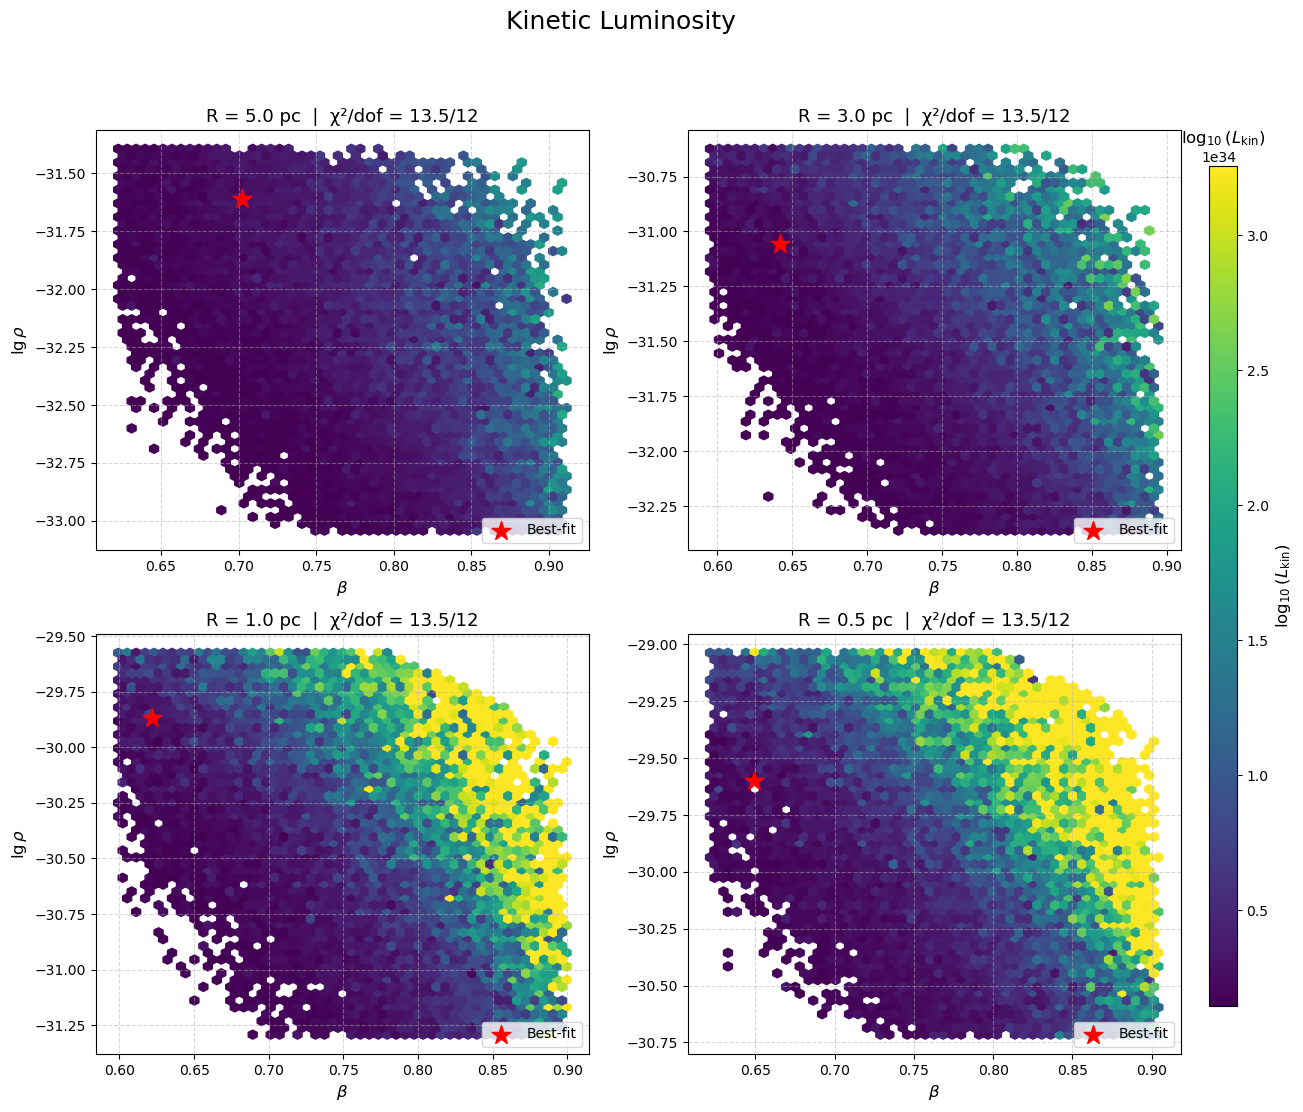
\includegraphics[width=0.5\linewidth]{electron_kin.png}
        \caption{Electrons' kinetic luminosity for all samples within 1-$\sigma$ statistical uncertainties.}
        \label{fig:sub1}
\end{figure}
\end{frame}
%--------------------------------------------------------------
\begin{frame}{Backup page 2}
\begin{figure}[ht]
    \centering
        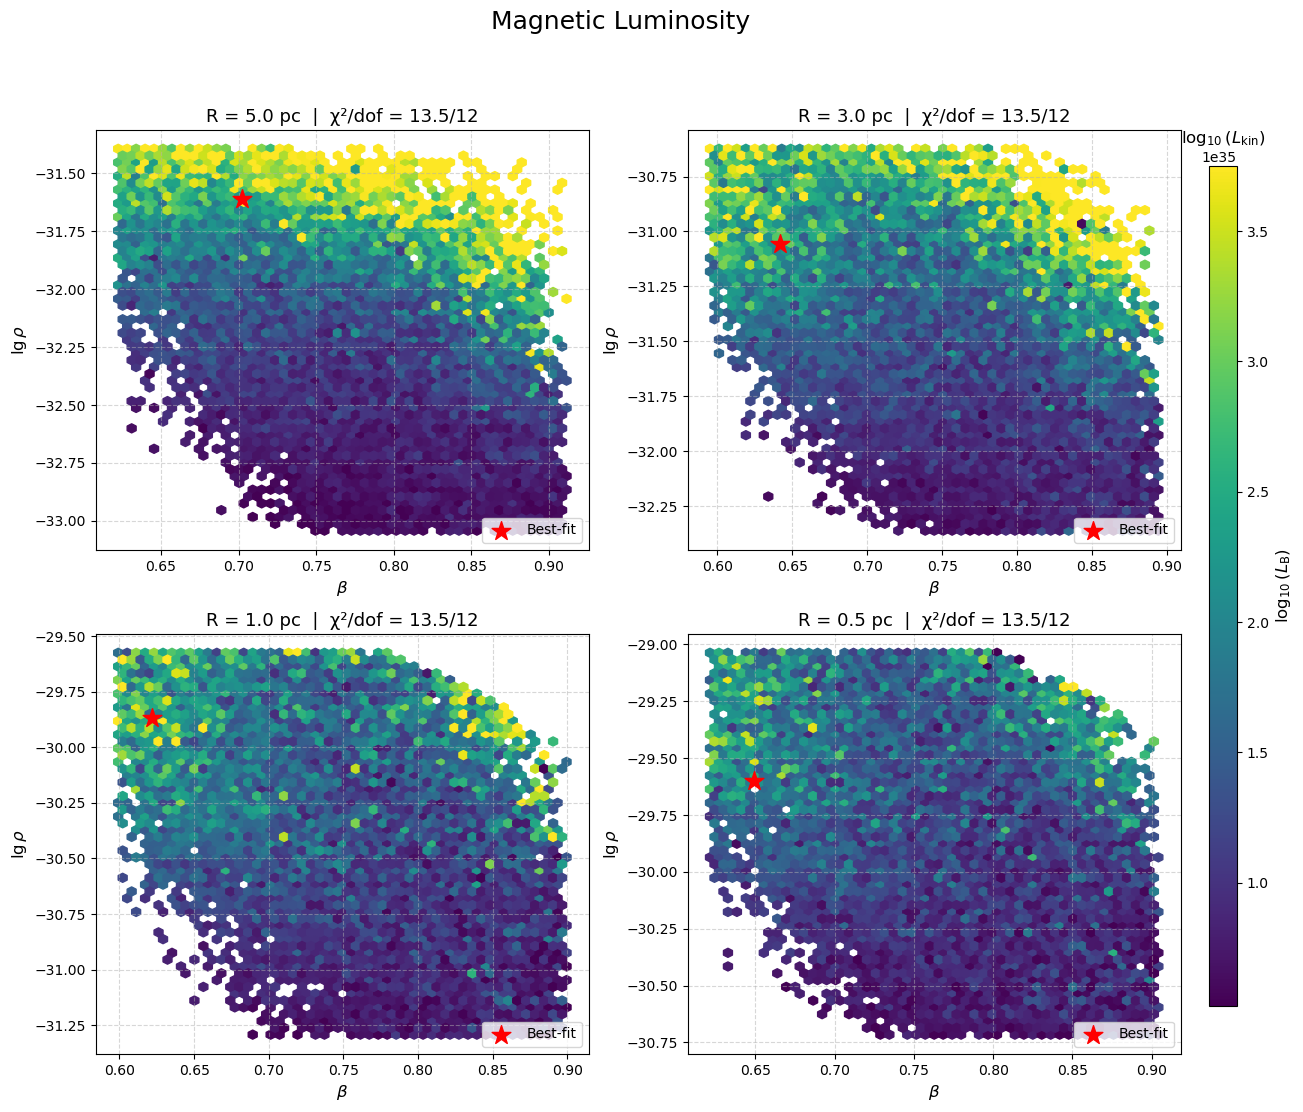
\includegraphics[width=0.5\linewidth]{mag.png}
        \caption{Magnetic luminosity for all samples within 1-$\sigma$ statistical uncertainties.}
        \label{fig:sub1}
\end{figure}
\end{frame}

%--------------------------------------------------------------
\begin{frame}{Backup page 3}
    \begin{figure}[ht]
    \centering
    % 使用 subfigure 环境并指定 [t] 选项
    \begin{subfigure}[t]{0.4\linewidth}
        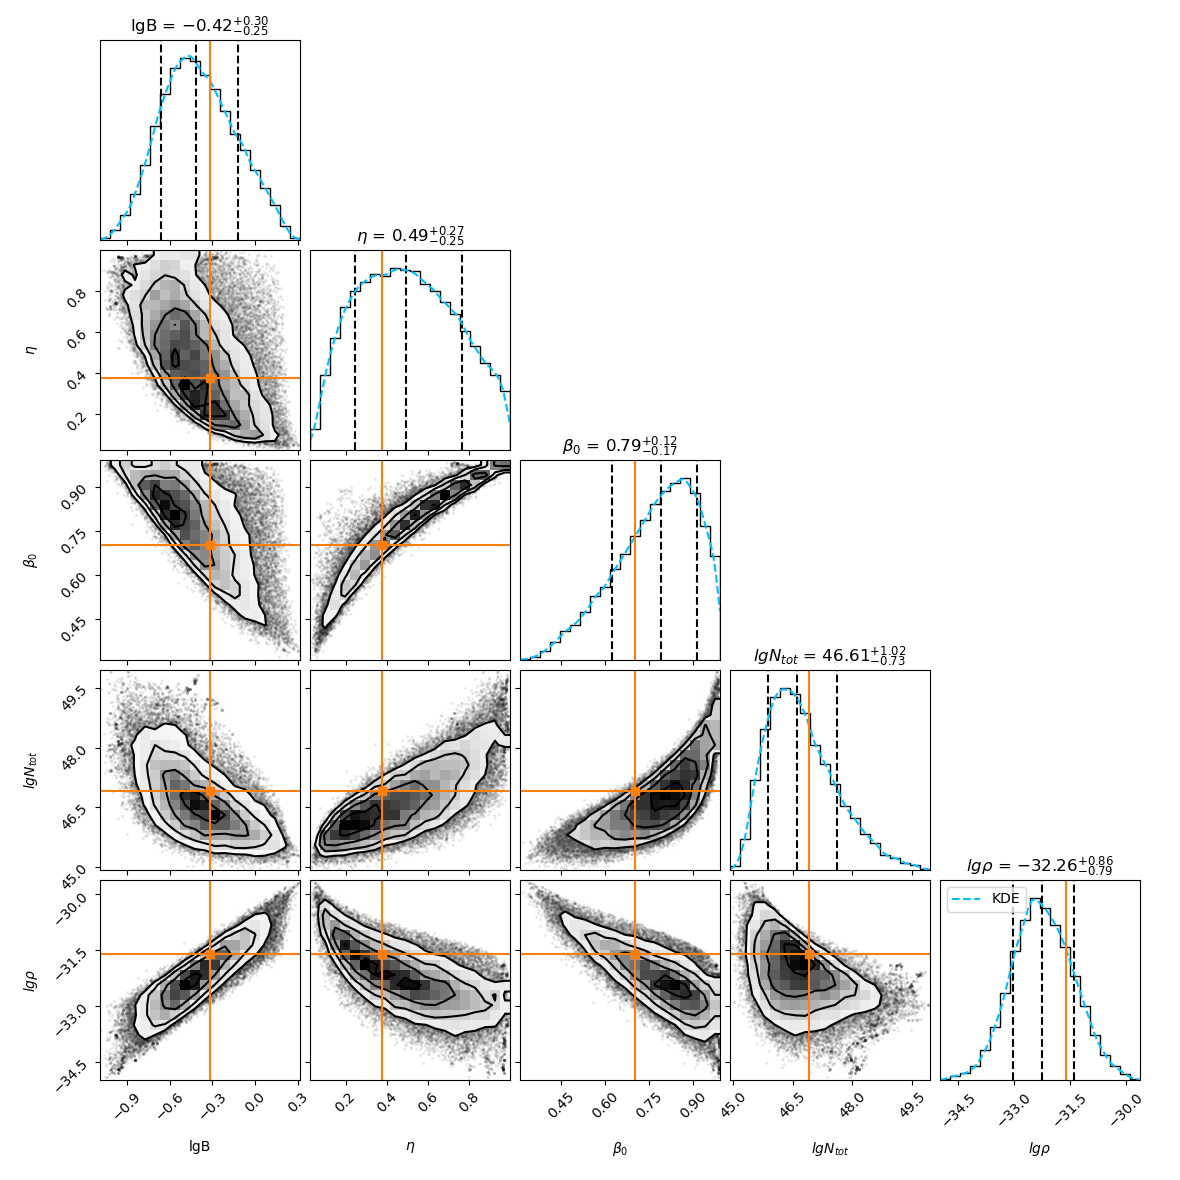
\includegraphics[width=\linewidth]{5pc.png}
        \caption{Corner plots for $R_{\rm jet}$ = 5 pc.}
        \label{fig:sub1}
    \end{subfigure}%
    \hfill % 在子图之间添加弹性的水平空间
    \begin{subfigure}[t]{0.4\linewidth}
        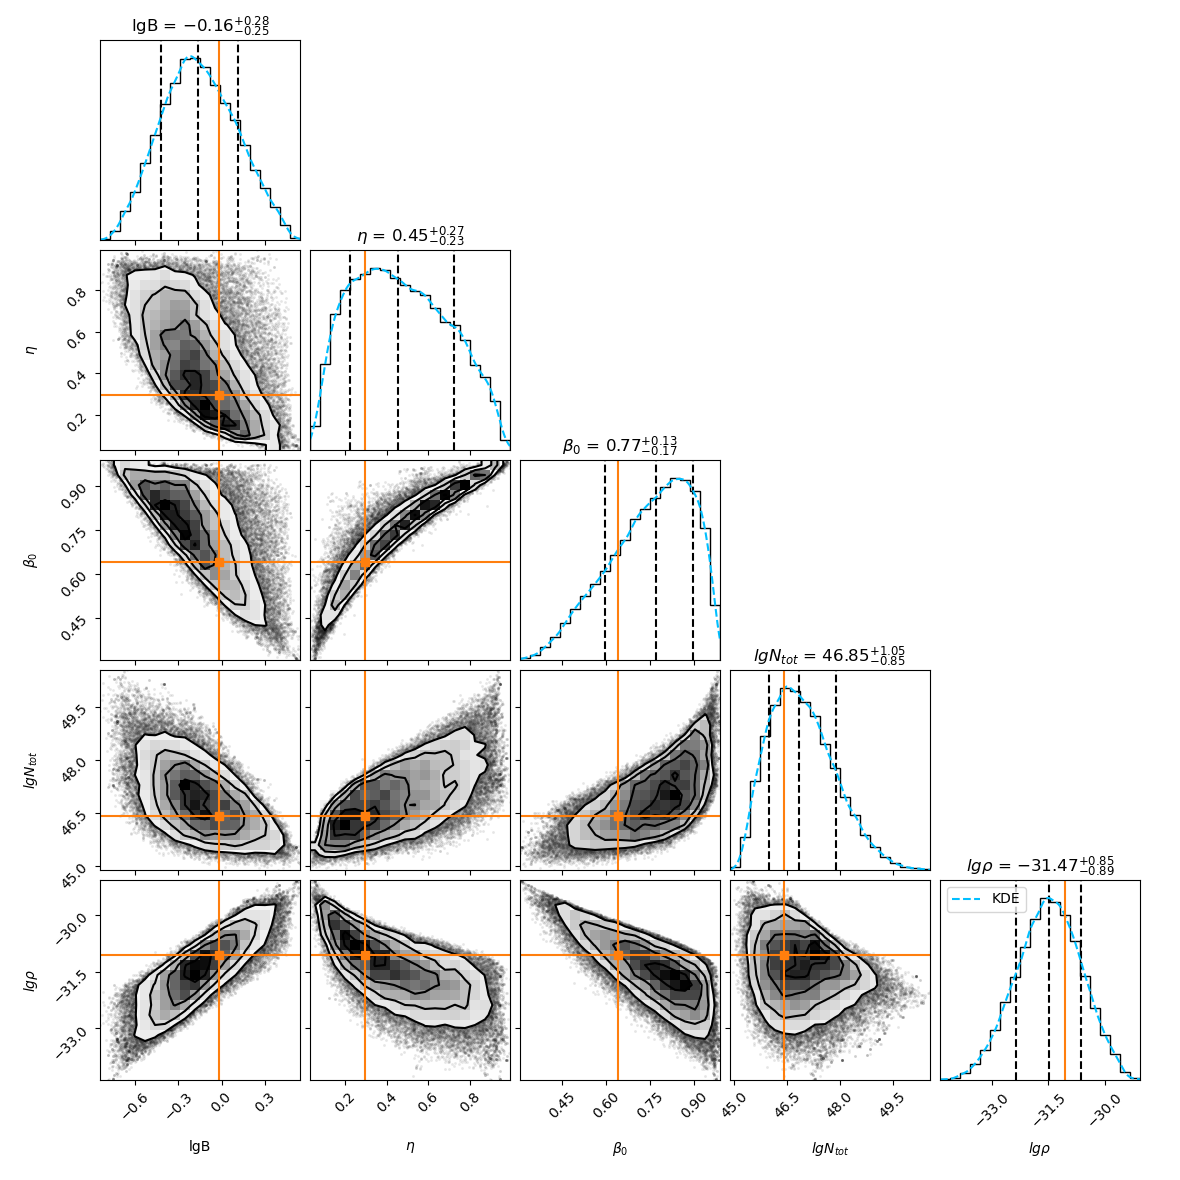
\includegraphics[width=\linewidth]{3pc.png}
        \caption{Corner plots for $R_{\rm jet}$ = 3 pc.}
        \label{fig:sub2}
    \end{subfigure}%
    \end{figure}
\end{frame}
%--------------------------------------------------------------
\begin{frame}{Backup page 4}
    \begin{block}{Details for the equation}
        \begin{itemize}
            \item SHA term: $\langle \overline{\frac{\Delta \gamma^2}{\Delta t} }\rangle_{\rm SHA} = \frac{\int_{0}^{R_{\rm jet}}2\pi r\langle \frac{\Delta \gamma^2}{\Delta t} \rangle_{\rm SHA} dr}{\pi R_{\rm jet}^2} = \frac{2}{15}\overline{\Gamma_{\rm j}^4}\left(\frac{\beta_0}{\eta R_{\rm jet}}\right)^2c^2\tau_{\rm sc}\gamma^2.$\\
            $\langle \overline{\frac{\Delta \gamma}{\Delta t}} \rangle_{\rm SHA} = \frac{\int_{0}^{R_{\rm jet}}2\pi r\langle \frac{\Delta \gamma}{\Delta t} \rangle_{\rm SHA} dr}{\pi R_{\rm jet}^2},\quad$ $\langle \frac{\Delta \gamma}{\Delta t} \rangle = \frac{1}{2\gamma^2}\frac{\partial}{\partial \gamma}\left[ \gamma^2 \langle\frac{\Delta \gamma^2}{\Delta t}\rangle \right]\,.$

            \item Radiative cooling: $\langle \dot{\gamma_c} \rangle=-\frac{\sigma_{\rm T}B_0^2\gamma^2}{6 \pi m_{\rm e} c}(1+\rm X)$, $\rm X$=$\frac{u_{\rm rad}}{u_{\rm B}}\,.$

            \item Diffusive escape: $t_{\rm esc}=\frac{R_{\rm jet}^2}{2\kappa}$, $\kappa = \frac{c \lambda}{3}\,.$

            \item STA term: $\langle \frac{\Delta \gamma^2}{\Delta t} \rangle_{\rm STA}=\frac{\Gamma_{\rm A}^4\beta_{\rm A}^2 \gamma^2}{\tau_{\rm sc}}\,.$

            \item The injection energy ($\gamma_{\rm eq}$) is defined as where $\langle \frac{\Delta \gamma}{\Delta t} \rangle_{\rm STA}$ = $\langle \frac{\Delta \gamma}{\Delta t} \rangle_{\rm SHA}$:\\ If $\gamma$<$\gamma_{\rm eq}$: STA dominates, while SHA electrons take over;\\
            $\gamma_{\rm rsn}$ is defined as where $r_{\rm L}$ = $\Lambda_{\rm max}$:\\
            If $\gamma$>$\gamma_{\rm rsn}$, $\lambda$ would increase sharply due to the loss of low-order wave-particle resonance.

            \item See \href{https://arxiv.org/abs/2507.02763}{Wan et al., 2025} for the complete derivation.
              
        \end{itemize}
    \end{block}
\end{frame}
%--------------------------------------------------------------

\end{document}
